% tudscrartcl inludes:
%	- koma-scipt
%	- typearea
%	- scrlayer-scrpage
%	- scrbase
%	- kvsetkeys
%	- etoolbox
%	- geometry
%	- textcase
%	- trimspaces
%	- graphicx
%	- xcolor
%	- environ
% manipulation via: \PassOptionsToPackage{option}{package}
\documentclass[ngerman]{tudscrartcl}
	\setlength{\parindent}{0pt}
	\setlength{\parskip}{10pt}
%%	\setlength{\baselineskip}{value}			% 1.0-single, 1.3-one and a half, 1.6-double

% corporate design demands the OpenSans package % needs lualatex
\usepackage{fontspec}
	\setmainfont[
				 Ligatures		= TeX,
				 ItalicFont 	= OpenSans-Italic,
				 BoldFont		= OpenSans-Bold,
				 BoldItalicFont = OpenSans-BoldItalic
				 ]{OpenSans-Regular}

% standard font incl. special letter
%\usepackage[utf8]{inputenc}

% set german as native language
\usepackage{babel}
\usepackage{ziffer}

% fits block type settings
\usepackage{microtype}

% consitent underlining
\usepackage{ulem}

% utilise \captionof{}{}
\usepackage{capt-of}

% introduces enumerations, itemisations and descriptions
\usepackage{enumerate}
%\usepackage{enumitem}
%	\noitemsep

% math environment
\usepackage{amsmath}
\usepackage{amsfonts}
\usepackage{amssymb}
%\DeclareMathSizes{18}{18}{18}{18}
%\usepackage[scaled=2]{helvet}

% SI units
\usepackage{siunitx}
	\sisetup{
%		list-final-separator	= {und schließlich},
%		list-pair-separator		= {und},
%		range-phrase			= {--},
%		range-units				= {single},
%		output-decimal-marker	= {,},
		locale					= {DE},
		input-decimal-markers	= {,},
		input-ignore			= {.},
		group-separator			= {\,},
%		group-minimum-digits	= {3}
		}

% clean tables
\usepackage{multicol}
\usepackage{multirow}
\usepackage{array}
\usepackage{tabularx}
	\newcolumntype{Y}{>{\centering\arraybackslash}X}
%	\def\tabularxcolumn#1{m{#1}}
%\usepackage{dcolumn}
%	\newcolumntype{d}[1]{D{.}{.}{#1}}
	\renewcommand{\arraystretch}{1.5}
\usepackage{booktabs}

% demands casted fig and tab to appear before the next section starts
\usepackage[section]{placeins}

% glossary, acronyms, sorting and indexing
\usepackage[
			acronym,
			toc,
			section,
%			style=altlist
%			automake,
			]{glossaries}
	\newglossary[slg]{symbolslist}{syi}{syg}{Formelzeichen}
	\makeglossaries

% links in toc - always load at the end
\usepackage[hidelinks]{hyperref}

% to imbed picturs in the text
\usepackage{wrapfig} 
%\usepackage{floatflt}

% to write reaction equations
\usepackage [version=3] {mhchem}



		% \input imports commands like written driectly
%============================================================================================================

% acronyms
\newacronym{tud}{TUD}{Technische Universität Dresden}
\newacronym{akr}{AKR-2}{Ausbildungs- und Forschungsreaktors}
\newacronym{ba}{BA}{Betriebsanweisung}
\newacronym{sus}{SuS-System}{Steuerungs- und Schutzsystem}
\newacronym{vk}{VK}{Verriegelungskreis}


% symbols
\newglossaryentry{symb:n}{
	name=$n$,
	description={Neutronendichte (proportional zu Neutronenflussdichte $ \phi $, Zahl der Neutronen $ N $, Reaktorleistung $ P $)},
	sort=symboln,
	type=symbolslist
}
\newglossaryentry{symb:k}{
	name=$k$,
	description={Multiplikationsfaktor},
	sort=symbolk,
	type=symbolslist
}
\newglossaryentry{symb:rho}{
	name=$\rho$,
	description={Reaktivität $ \rho = (k-1)\ /\ k $},
	sort=symbolrho,
	type=symbolslist
}
\newglossaryentry{symb:beta}{
	name=$\beta$,
	description={Gesamtanteil der verzögerten Neutronen für U-235: $ \beta = 0,641 \si{\percent} $},
	sort=symbolbeta,
	type=symbolslist
}
\newglossaryentry{symb:l}{
	name=$l$,
	description={Neutronen-Generationsdauer $ l^{\star} = l / k $},
	sort=symboll,
	type=symbolslist
}
\newglossaryentry{symb:lambda}{
	name=$\lambda$,
	description={mittlere Zerfallskonstante der Mutterkerne verzögerter Neutronen},
	sort=symbollambda,
	type=symbolslist
}
\newglossaryentry{symb:C}{
	name=$C$,
	description={Konzentration der Mutterkerne verzögerter Neutronen},
	sort=symbolC,
	type=symbolslist
}
\newglossaryentry{symb:T}{
	name=$T$,
	description={Reaktorperiode, d.h. Zeitdauer, in der sich die Neutronenflussdichte bzw. die Reaktorleistung um den Faktor $ e = 2,71 $ ändert},
	sort=symbolT,
	type=symbolslist
}


% glossary
%\newglossaryentry{test}{name={Test}, description={A test entry}}
%============================================================================================================

\begin{document}
	% --- Frontpage -----------------------------------------------------------------------------------------
	\TUDoption{cd}{lightcolor}%false/true,light-/bar-/bi-/full-/color
	\TUDoption{cdhead}{wide,bicolor}%false/true,heavy,no-/light-/bar-/bi-/color,slim/wide,no-/date
%	\TUDoption{cdmath}{true}
%	\TUDoption{cdchapter}{true}
	
	\faculty{Fakultät Maschinenwesen}
%	\department{}
	\institute{Institut für Energietechnik}
	\chair{Professur für Wasserstoff- und Kernenergietechnik}
	\date{\today}
	\author{Dr. C. Lange}
	\title{Reaktorpraktikum - Versuch: Bragg-Streuung}
	\headlogo{pics/Logo_WKET_weiss.eps}
	
	\pagenumbering{gobble}
	\maketitle
	
	\begin{figure*}[!htb]
		\centering
		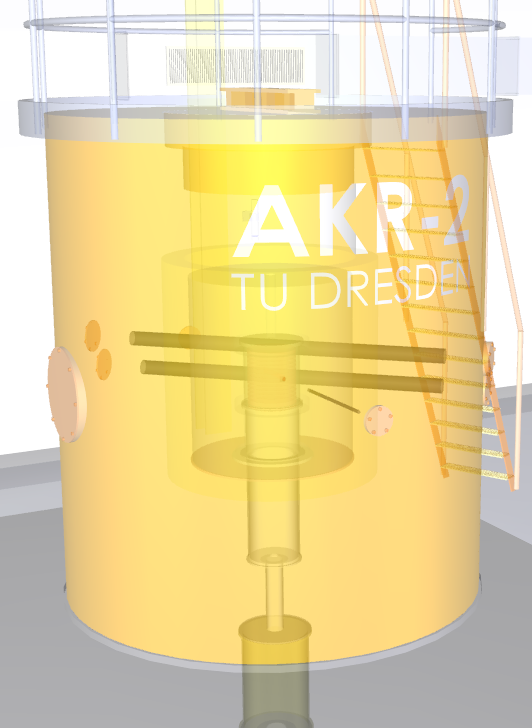
\includegraphics[width=0.6\linewidth]{pics/akr_model.png}
	\end{figure*}
	
	\newpage
	
	% --- ToC -----------------------------------------------------------------------------------------------
	\pagenumbering{arabic}
	\tableofcontents	% needs also the pages before the toc; how to?
	\newpage
	
	% --- Acronyms ------------------------------------------------------------------------------------------
	\printglossary[type=\acronymtype, title=Akronyme, nonumberlist]
	\printglossary[type=symbolslist, nonumberlist]
	\glsaddall
	\newpage
	
	% --- Inhalt --------------------------------------------------------------------------------------------
	\section{Ziele und Motivation}

Im folgenden Versuch soll das Phänomen der Bragg-Streuung an Neutronen untersucht werden. Im Falle von Röntgenstrahlung stellt sie eine wohl bekannte Beobachtung dar. Aufgrund des Welle-Teilchen-Dualismuses kann dieser Effekt auch mit "klassischen" Teilchen wie Elektronen beobachtet werden.
Dass ein solches Phänomen jedoch auch mit Objekten, die noch aus mehreren Teilchenarten zusammengesetzt sind, auch möglich ist, scheint zunächst schwer vorstellbar. Dass es funktioniert, wollen wir mit dem folgenden Versuch zeigen. Dabei kommt auch wieder eindrucksvoll der Welle-Teilchen-Dualismus zum Tragen, der offensichtlich auch für Neutronen funktioniert. Eine Streuung an Kristallatomen ist nur im Wellenbild erklärbar, während der Nachweis der Neutronen über die Absorption durch Zählgasatome nur über eine Beschreibung des Neutrons als Teilchen erklärbar ist. 

\subsubsection{Geschichte}

1932 entdeckte J. Chadwick das von E. Rutherford bereits 1920 vorausgesagte Neutron. Grundlage für seine Entdeckung war ein Experiment, welches von Walther Bothe und seinem Studenten Herbert Becker durchgeführt wurde, bei dem sie Beryllium mit Alphastrahlung beschossen. Sie hielten die bei der Reaktion entstandene stark durchdringende und energiereiche Strahlung, da sie auch nicht auf äußere elektrische Felder reagierte, fälschlicherweise für Gammastrahlung. Doch als Endprodukt entstand nicht wie vorher erwartet Bor, sondern Kohlenstoff.

Die entdeckte Strahlung war viel energiereicher als jede zuvor entdeckte Gammastrahlung und so kamen Zweifel daran auf, ob es sich wirklich Gammastrahlung handelt. Chadwick, der nicht überzeugt von der Erklärung mit der Gammastrahlung war, entwickelte eine schnell eine Reihe von Experimenten, in denen sich herausstellte, dass es sich bei der Beryllium-Strahlung um ungeladene Teilchen mit der ungefähren Masse von Protonen handeln muss. Für diese Entdeckung erhielt er 1935 den Nobelpreis für Physik.
Aufgrund des Welle-Teilchen-Dualismus der Neutronen und der Entwicklung der Elektronenbeugung, konnte H. Halban 1936 zeigen, dass Neutronenbeugung in der Theorie möglich ist. Der experimentelle Beweis blieb aber noch aus, da zu dieser Zeit die Neutronenquellen noch keine starken Flüsse erzeugen konnten. Mit der Entdeckung der Kernspaltung durch Lise Meitner und Otto Hahn im Jahre 1938 und der darauffolgenden Entwicklung der ersten Kernreaktoren, konnte erstmals 1944 ein wirklich starker Neutronenfluss generiert werden. Seitdem wurden zahlreiche Neutronenbeugungsexperimente durchgeführt. In den ersten paar Jahren konzentrierte man sich auf Beugungsversuche und fand heraus, dass sich inelastische Neutronenstreuung sehr gut zur Spektroskopie eignet. Dank der fehlenden Ladung können die Neutronen tief in Materie eindringen (interagieren nur mit den Kernen) und werden nicht von Oberflächeneffekten beeinflusst, was zum Beispiel ein Nachteil der Röntgenstrahlung ist.

	\section{Aufgabenstellung}
	\section{Theorie}

\subsection{Detektion der Neutronen}

genutzte Quellen: \cite{PRuD,He3_vacutec}

Zur Detektion von ionisierender Strahlung werden oft Zählrohre verwendet. Es existieren Ionisationskammern,  Proportional-  und Geiger-Müller-Zählrohre. Sie folgen alle einem ähnlichen Aufbau, arbeiten jedoch bei unterschiedlichen Spannungen.  Dies kann an der Zählrohrcharakteristik verdeutlicht werden. Sie zeigt die Abhängigkeit der Anzahl der gemessenen Impulse von der  Zählrohrspannung. Zu sehen sind verschiedene Bereiche:

%\begin {wrapfigure} [Zeilenanzahl, die um Bild fließen sollen] {Position, l = links, r = rechts} [Randüberhang] {Breite}

\begin{wrapfigure} {R} {10cm}
	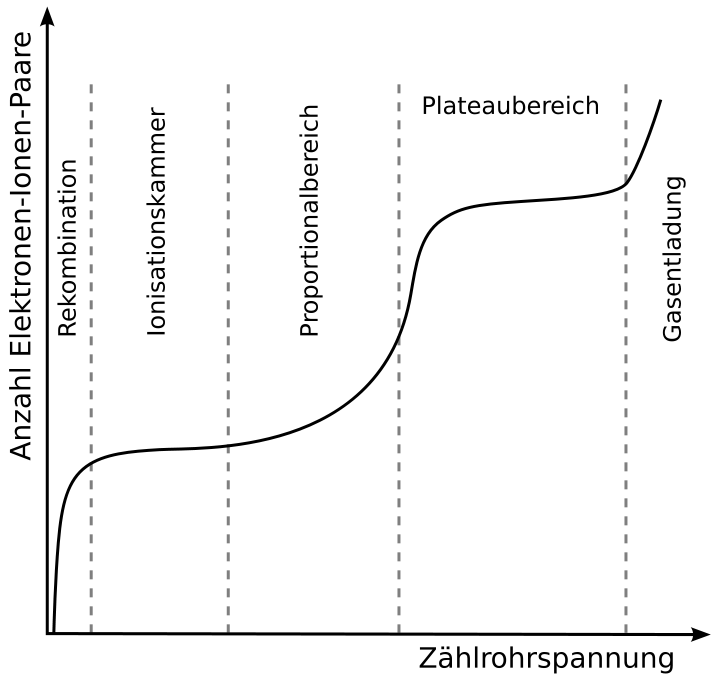
\includegraphics [width=10cm] {pics/Kennlinie_Zaehlrohr.png}
	\caption {Zählrohrcharakteristik\protect\footnotemark }
\end{wrapfigure}
\footnotetext {Bild aus: \url{https://upload.wikimedia.org/wikipedia/commons/thumb/d/d3/Kennlinie_Zaehlrohr-GER.svg/720px-Kennlinie_Zaehlrohr-GER.svg.png}  [06.06.2018 21:31 Uhr]}

%\begin{floatingfigure} [r] {10 cm}
%	\centering
%	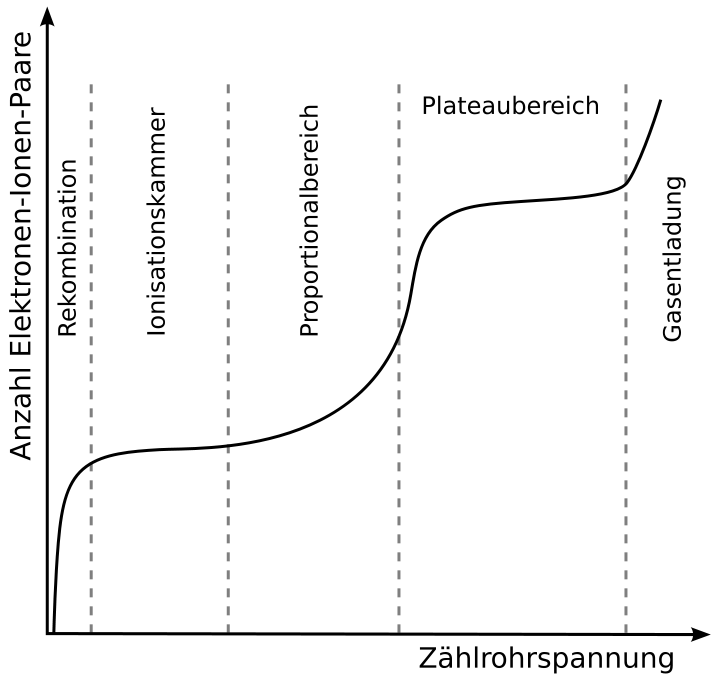
\includegraphics {pics/Kennlinie_Zaehlrohr.png}
%	\caption {Zählrohrcharakteristik}
%\end{floatingfigure}

\begin{description}
	\item[Bereich I: Rekombination] Die Spannung zwischen Kathode und Anode ist so gering, dass ein Teil der Elektronen auf dem Weg zur Anode mit den Ionen im Zählgas rekombinieren. Oft ist es hier nicht einmal möglich, eine Messung durchzuführen.  
	
\end{description}
\begin{description}

	\item[Bereich II: Sättigungsbereich] Die Spannung ist groß genug, sodass alle durch die Strahlung direkt erzeugten Elektronen (Primärelektronen) die Anode erreichen. 
	
	
	In diesem Spannungsbereich werden Ionisationskammern betrieben. Anhand der erreichten Impulshöhe/Ladungsmenge lassen sich Rückschlüsse auf die Art und Energie der eingetroffenen Teilchen schließen. 
	
	\item[Bereich III: Proportionalbereich] Wird die Spannung weiter erhöht, wird es den beschleunigten Primärelektronen möglich, weitere Gasmoleküle durch Zusammenstoß zu ionisieren (Stoßionisation), wodurch sogenannte Sekundärelektronen entstehen. Die stattfindende Sekundärionisation ist in diesem Bereich proportional zur primären Ionisation. Dadurch ist es auch hier möglich, Rückschlüsse auf Art und Energie der einfallenden Teilchen zu ziehen. In diesem Bereich werden Proportionalzählerrohre wie der in diesem Experiment verwendete He3-Detektor betrieben.
	
	\item [Bereich IV: Auslösch- oder Plateaubereich] Durch weitere Erhöhung der Spannung erreicht man einen Bereich, in dem die Sekundärionisation Lawinencharakter annimmt. Während es im Bereich III nur den energiereicheren Elektronen möglich war, Sekundärelektronen zu erzeugen, produziert nun jedes Primärelektron produziert hierbei eine Lawine von Sekundärelektronen. Daher erhöht sich die Anzahl der gezählten Impulse nicht mehr merklich, wenn die Spannung weiter steigt, da alle einfallenden Teilchen detektiert werden. Es ist nur noch eine reine Zählung möglich, Art und Energie der einfallenden Teilchen können nicht mehr bestimmt werden. In diesem Spannungsbereich werden Geiger-Müller-Zählrohre betrieben. 
	\item [Bereich V: Dauerentladung]
\end{description}

Zur Messung der gestreuten Neutronen wird ein Helium3 (3He)- Detektor verwendet. Bei Neutronen handelt es sich um ungeladene Teilchen. Um sie nachweisen zu können, müssen aus ihnen erst durch Wechselwirkung mit Materie geladene Teilchen erzeugt werden, die sich mithilfe eines elektrischen Feldes beschleunigen und schließlich messen lassen. Im vorliegende Detektor wird dies durch eine Wechselwirkung des He3 mit den Neutronen realisiert, die bei Neutronenenergien unter 20 MeV stattfindet: 
\ce{n + ^3He -> p + ^3He}
Der Detektor selbst arbeitet als Proportionalzählrohr. Dies besteht aus einem metallischen, zylindrischen Rohr und einem auf der Zylinderachse befindlichen Metalldraht. Zwischen dem Rohr (Kathode) und dem Metalldraht (Anode) wird eine Spannung angelegt, sodass ein elektrisches Feld im Inneren des Rohrs entsteht. Das Rohr selbst ist mit einem Zählgas gefüllt, in diesem Fall mit Helium-3. Die Neutronen wechselwirken mit dem Helium wie oben beschrieben und erzeugen ein Proton und ein Tritiumatom. Diese geladenen Teilchen sind nun in der Lage, Gasatome zu ionisieren. Dadurch werden Elektronen frei, die zur Anode wandern. Die Arbeitsspannung des elektrischen Feldes ist entsprechend so gewählt, dass einige Elektronen in der Lage sind, weitere Gasatome zu ionisieren, wodurch Sekundärelektronen entstehen. Die Elektronen, die die Anode erreichen, erzeugen dort einen Strompuls, der über einen Widerstand in eine Spannung umgewandelt wird, die dann elektronisch weiterverarbeitet und gezählt werden kann. 

Die Effizienz des Detektors berechnet sich nach näherungsweise nach folgender Formel:

\begin{equation}
	\epsilon = 1-e^{-\sum_{a} (E) L}
\end{equation}

Für eine exakte Messung mittels des He3-Detektors muss eine günstige Arbeitsspannung gefunden werden. In der oben erwähnten Zählrohrcharakteristik ist der generelle Spannungsverlauf im Proportionalbereich ersichtlich. Wir wollen im Folgenden etwas genauer darauf eingehen. 




%\begin{itemize}
%	\item Brennstoffabbrand,
%	\item Vergiftung des Brennstoffs oder
%	\item Temperatureffekte
%\end{itemize}

%während der Versuchsdauer praktisch vernachlässigt werden können. Damit entspricht jeder Start eines solchen Nullleistungsreaktors einem Kaltstart eines Leistungsreaktors hinsichtlich des nuklearen Teils dieser Anlage.



	\section{Durchführung}
	\section{Auswertung}
	\section{Hinweise}
	\section{Fragen} % \include comes with clearpage commands, etc.
	\newpage
	
	% --- Appendix ------------------------------------------------------------------------------------------
		
	\listoffigures
	
	\listoftables
	
	\nocite{*}
	
	\bibliographystyle{unsrtdin}
	\bibliography{latex-files/prakt_reaktorstart}
\end{document}